% %%%%%%%%%%%%%%%%%%%%%%%%%%%%%%%%%%%%%%%%%%%%%%%%%%%%%%%%%%%%%%%%%%%%%%
% Dummy Chapter:
% %%%%%%%%%%%%%%%%%%%%%%%%%%%%%%%%%%%%%%%%%%%%%%%%%%%%%%%%%%%%%%%%%%%%%%

% %%%%%%%%%%%%%%%%%%%%%%%%%%%%%%%%%%%%%%%%%%%%%%%%%%%%%%%%%%%%%%%%%%%%%%
% The Introduction:
% %%%%%%%%%%%%%%%%%%%%%%%%%%%%%%%%%%%%%%%%%%%%%%%%%%%%%%%%%%%%%%%%%%%%%%
\fancychapter{Technical Implementations}
\label{cap:chapter}

\textit{As the first part of this thesis' work development, I implemented and coded the hardware adaptations and software protocols for the real-time behavioral control and stimulus presentation to be used in the experiments with the open-source arduino-based system Bpod, by adapting the previously used microkernel-based system Bcontrol. This implied the ensurement of a syncronized graphical user interface, the comunication between a governing machine, a microscopy apparatus, a stimuli monitor and a bpod device, within minimal processing time, as well as different states matrices and protocols for each stimulation type - RF mapping, tuning mapping and SM properties investigation.
Moreover, the system also required proper functionality within the software controling the two-photon microscope, which was enabled by proper understanding of the trigger and configuration requirements of the software ScanImage.}

\section{System's scheme}
\label{sec:sectiona}

The experimental procedure of visual stimuli display involved four main components in communication of parameters, configurations and triggered synchronization: A governing machine and a stimulus display matlab instances, a Bpod device and the set of two-photon laser microscopy appliances and software. 

\begin{figure}[H]
	\centering
		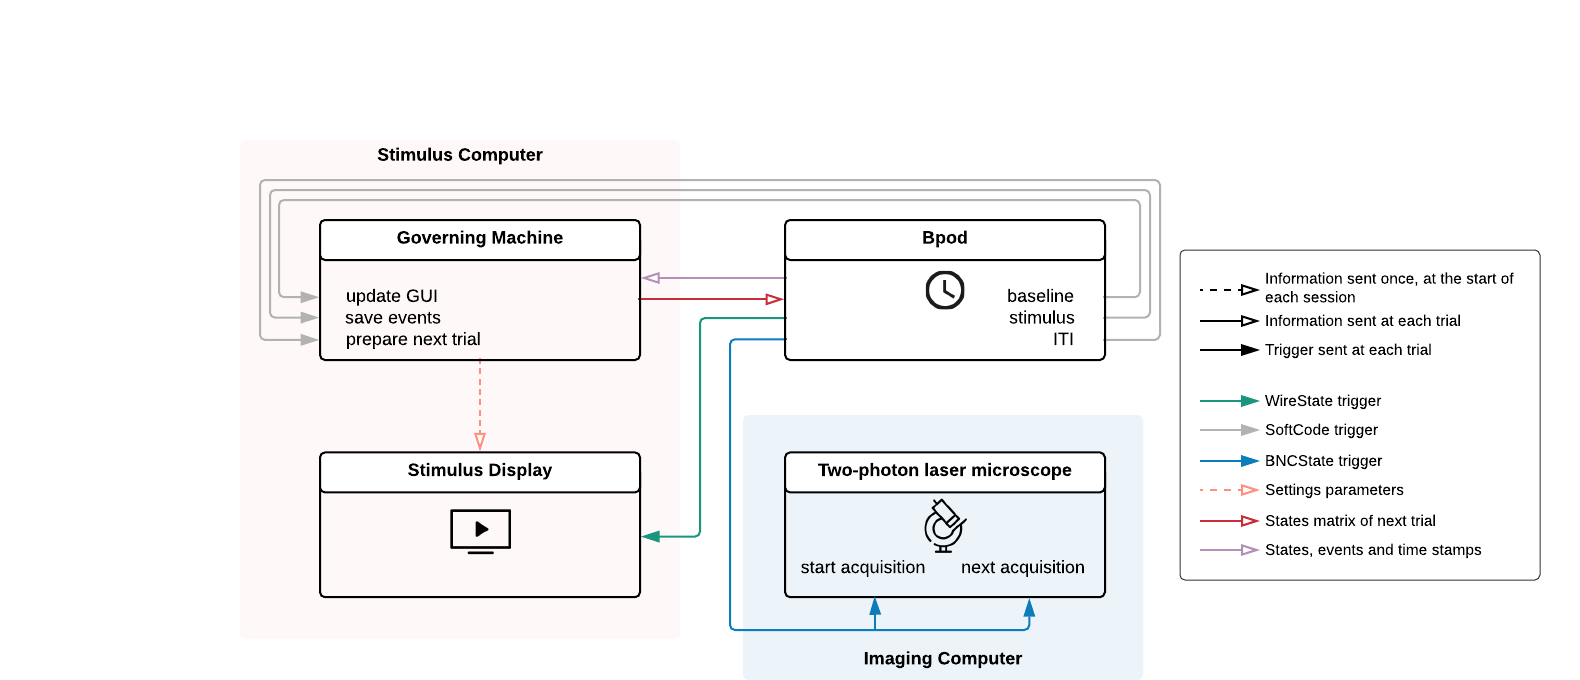
\includegraphics[width=1\linewidth]{3.Chapter/systemtechnical.png}
	\caption[c1]{Setup and connections scheme of devices used for stimuli presentation and real-time imaging.}
	\label{fig:systemtechnical}
\end{figure}

The governing machine and the stimulus display were controlled by one of the computers, called here stimulus computer.

The governing machine held the Graphical User Interface (GUI) as well as all of the computations and running protocols with Bpod's software for saving the stimuli settings and preparing the stimuli configurations and states matrices for the different trials. 

The stimulus was displayed in a second monitor connected to this stimulus computer and operated within a second matlab instance of routines coded with Psychtoolbox software for interfacing between Matlab and the computer screen. This Matlab instance loaded, at the beginning of the session, all of the stimuli settings that were saved in the bpod's Matlab instance. With a counter, the script iterated the full trials structure, displaying the applicable stimuli at the proper times. This timing synchronization was enabled by triggers received in a NI-DAQ data acquisition board. 

The bpod apparatus produced these triggers, connected to the system and taking advantage of a precise internal clock. Having received each trial's state-matrix specifications from the governing machine with enough buffer time, bpod produced the appropriately timed states - the main ones being the baseline, the stimulus and the ITI - and sent the required triggers at each stage. At each trial, in the beginning of the baseline period, a trigger was sent to the governing machine to update the GUI to show the current trial stimuli specifications; during the stimulus presentation, another trigger was sent to save the events of the previous trial and during the ITI an instruction was sent for the governing machine to prepare the next trial by computing the next states matrix with the new trial's stimuli configurations. Bpod also sent, at the beginning of the stimulus display state, the trigger for the stimulus computer second matlab instance to display the loaded and prepared stimulus in the screen visualized by the animal. Finally, at the beginning of the baseline and in the end of the ITI of the proper trials, a trigger was sent to the called imaging computer that held the software controlling the two-photon laser microscope for respectively starting and afterwards completing and proceeding to the next scanning acquisition. 

The two-photon laser microscope had different components: The laser apparatus with the mirrors, lenses, beam-splitter and remaining light path enforcers; the objective enabling both a bright field and a two-photon configurations; the synchronization device, a NI-DAQ data acquisition board for receiving Bpod's triggers, and finally the imaging computer that operated the controlling software application ScanImage 4 for laser scanning microscopy. This was also the computer that saved the raw image sets acquired from the two-photon scannings at each protocol session.

The information sent and triggers used the different physical wiring possibilities: Firstly, \textit{SoftCodes} were sent from bpod to the governing machine's computer. These are code that go via the USB port that connected these devices. From bpod to the stimulus display NI-DAQ board, \textit{WireStates} were used, from wire ports in bpod, and, to the two-photon NI-DAQ board, \textit{BNCState} triggers were sent, from bpod's BNC ports. On the other hand, the information about states, events and trial time stamps was sent at each trial via USB from the Bpod device to the bpod's governing machine matlab instance and then saved with its own software. 
From the governing machine, information was sent as the following trial's state matrix, to the bpod device also via USB (Softcode) and the next trial's settings were sent to the stimulus display matlab instance by saving them at the beggining of  each protocol session in a file that was then loaded in the stimulus display matlab before starting the session.
\section{Bpod}
\label{sec:sectionb}
\subsection{Motivation and previous system}
\label{subsec:subasectionB}

Bpod encompasses a flexible open-source platform for developing stimuli presentation, behavioural protocol and reinforcement experiments. The system builds on a parallel processing model, software functions are written in Matlab/Python and the firmware builds on Arduino language. The system was develloped in Kepecs Lab [REFERENCES] at Cold Spring Harbor Laboratory and is currently maintained by Sanworks LLC, a company focused on open source neuroscience tools.

The main capability of the system is its precise time measuring feature. In imaging and even more so in electrophysiology animal experiments, it is paramount to control and synchronize the timings of stimuli presentation, behaviour/neuronal activity detection and states sequencing in the different setup compontents. Precise triggers from a governing machine to a brain activity measurement device - the two-photon setup, in this case -, to a stimuli display - visual or not - or behavioural gadgets allows reliable functional brain mappings, and appropriate analysis and interpretation of an animal's brain or physical responses.


Prior to this implementation, the Cortical Circuits Lab was using B-control for mice's behavior measurement and finite states machine, a system developed by Brody Lab at Princeton University [REFERENCES]. In fact, Bpod builds on B-control's parallel processing design idea: the state machines for each trial are constructed in Matlab in a governing machine and executed in a separate device. For B-control, this is a separate microkernel real-time Linux computer. Bpod, on the other hand, uses an Arduino microcontroller network with finite state machine firmware for the real-time processing. This provides higher level software tools for adapting and constructing protocols, as well as a simpler, less expensive hardware solution.


Bpod entails two items: The device that provides the state machine substract, with a precise internal clock, output ports for TTL triggering, input ports, behavior ports with infrared photogates, LEDs and solenoid valves for dispensing liquids; and the software that, run in the governing machine, provides functions with which to code the states matrix, to equip the system with a GUI and the necessary supporting functions for each protocol and to implement functioning communication between the Bpod device and the other components - in  the case, the stimuli computer and the two-photon computer. 

The Bpod system presents the following five principal functionalities:

\begin{itemize}
\item Ensures the precise triggering between the Bpod device and the involved components - microscope set, stimuli screen and governing machine;
\item By enabling the implementation of a GUI interface, this equips the user with a practical way of setting the characteristics of the stimuli at the start of the experimental session;
\item The GUI also facilitates the monitoring of the stimuli presentation sequence at the same time as it is happening in a given session: the current trial with its correspondent stimuli properties is shown, as well as the appropriately timed states - baseline, stimuli presentation, ITI and auxiliary states - within the running protocol. Moreover, the states machine can be started - with the last submitted stimuli settings -, stopped, paused, continued or restarted by the user at any time, keeping the synchronization and . [GET IMAGE] 
\item Automatizes the saving of the data structures containing a session's stimuli sequences, as well as the time stamps related to the state matrix that was run, with the computer times for the start of each state or event leading to a state change.
\item Although not used during this work, as the experiments only regarded stimuli presentation, and because the animals were kept anaesthetized, minimizing the need for further controls, one of Bpod's main functionalities regards the measuring of the animal's behaviour. The state machine receives these discrete behavioral events and can rapidly respond by changing the animal's environment. For instance, by connecting Bpod to treadmills, one can measure a small animal running behaviour;  by connecting Bpod's appropriate ports to water valves connecting to drinking tubes, those can be controlled for implementing a reward system during reinforcement experiments; Bpod also detects the instant when discrete events happen. This can be used for example in decision making experiments: a snout entering a port or a tongue blocking a photogate can indicate an animal choices. High quality audio stimuli can also be produced with the integration of Psychtoolbox. These features deem the Bpod system a practical tool for various behavioral paradigms: two alternative forced choice (2AFC), go/no-go decisions, reaction time measurement, self-stimulation (repetition of physical movements), social value measurement, among other possibilities. 
\end{itemize}

The access to these functionalities is to be understood as provided that the user develops the programming protocols and optimizes it to meet the requirements that the experiment entails. Bpod system is not a ready to use package: it requires an understanding of the functions provided, Matlab or Phyton coding, and all of the hardware communication specifications in each protocol's case. More fundamentally, the user should have a clear planning of the specific communication scheme to use in their case, as well as of the GUI and states machine development and the important variable structures with the information to be produced, exchanged between components and saved. Documentation is available in [BPOD WIKI] and technical support can be found in the cooperative [BPOD FORUNS].

The development process started in a 45-days internship at the Cortical Circuits Lab in 2016, in which l adapted a stimuli presentation protocol from Bcontrol to Bpod, by familiarizing with both Bpod and B-control syntaxes and function environments. This work was carried with the mentorship of Leopoldo Petreanu and the guidance of Tiago Marques through the B-control environment protocol that he had developed and that the Laboratory had been using. The protocol enabled full-screen moving gratings or random dots, under different stimuli properties - timings, screen stimuli positioning, number of repetitions, luminosity values, gratings versus random dot stimuli type probability, orientation, direction, dots speed, density, coherence and size, gratings temporal and spatial frequency - in pseudo-randomized selections according to a general user's requirements with the possibility for fixating a seed, facilitating troubleshooting. At the time, this protocol was tested with the same stimuli Psychtoolbox code written for B-control. Since then it was further used in electrophysiology experiments in the Laboratory by the PhD student Gabriela Fiorze.

In this thesis' protocols development, I used  this previously coded and tested protocol as a basis. However, in this case, besides having to adapt the states machine, GUI, main and support functions from the governing machine, it was also necessary to develop new stimuli protocols with Psychtoolbox [REFERENCES] and to understand the triggers, ScanImage software [REFERENCES] and hardware connections made with the two-photon computer setup. Furthermore, at the time I used a Bpod State Machine device at version 0.5 that was switched at this point for version 0.9, with slight differences in hardware, as well as in the software functions and firmware.

In the following chapters I will go through the three protocols I developed for this thesis' experiments. For these, as in the originally developed Bpod protocol, I focused on the protocols user-friendliness, minimal processing time and in the flexibility of the code for both other similar experiments and for adaptations to other paradigms.

\subsection{Bpod Hardware implementation, specifications and alterations}
\label{subsec:subbsectionB}

The Bpod State Machine device runs on a Arduino Due 32-bit processor with 84MHz clock speed. The bill of materials can be found at the device's wiki [REFERENCES]. 


\begin{figure}[H] \centering 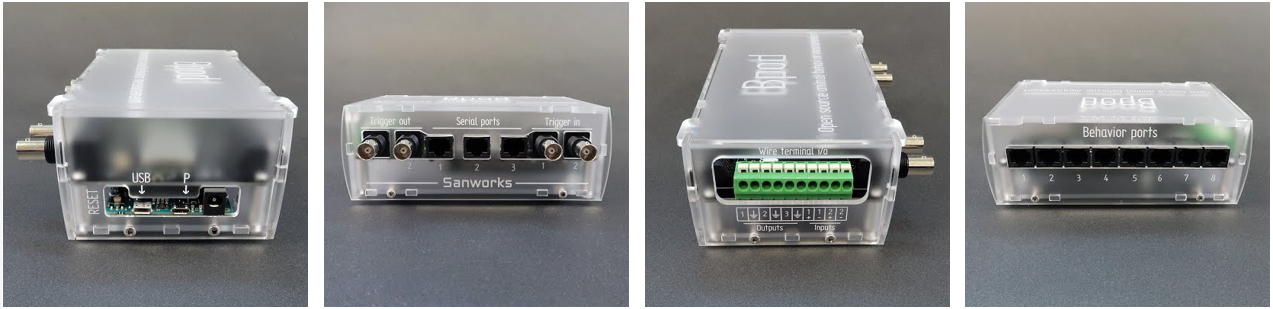
\includegraphics[width=16cm,height=16cm,keepaspectratio]{Figures/3.Chapter/bpodangles.png} 
\caption{Perspectives of Bpod State Machine device version 0.5, identical parts as in version 0.9, but with fully transparent box container design. Images from Sanworks Bpod wiki page [REFERENCES].} 
\end{figure}


Firstly, the device contains a 'reset' button to reset the device if necessary and two USB port jacks - an Arduino's native USB port to connect to the governing machine and a programming port for cases when it is necessary to re-upload Bpod's firmware. Moreover, there also is a power barrel jack for cases when the USB port is not supplying enough power to the device - this power jack was used in troubleshooting but, with the final setup, the power from the USB proved to be enough.


In Bpod, there are four BNC channels, two input and two output. The output channels are constructed to serve as 5V triggers, as Bpod can produce events and send triggers with TTL logic through them. These were initially used here to connect to the two-photon computer's NIDaQ board, one of them as a 'start acquisition' trigger and the other as a 'next acquisition' trigger. 

Bpod also has bare wire terminals, with TTL logic. The spring terminal channels are of two inputs (2.5V to 5V) and three outputs, all with the respective grounds. The outputs here are 3.3V TTL pulses. In this thesis work, I required one extra trigger port to be connected to a NiDAQ [THE WHITE THING]. This WHITE THING was by its turn controlling the stimuli screen. One of these wire channels was thus used to portray trigger pulses. For this, to be assured that there was sufficient voltage at this port (5V, according to the WHITE THING specifications [REFERENCE]), the Bpod circuit was altered in the Champalimaud Foudation IT platform with a 3.3V to 5V voltage amplifier at this wire output channel [HOW? CHECK].

Although not used in these experiments, the apparatus additionaly contains behavior study components: An ethernet that can connect to a lickometer or a nose port, as well as 8 behavior ports, each with an LED with software-adjustable intensity, a solenoid valve (12V, 150mA), and an infrared photogate. Also not necessary for these experiments, the device also contains serial ports that allow to connect it to other Arduino boards or modules that can be acquired from the same company.




%\section{Bpod}
\label{sec:sectionc}
\subsection{Motivation and previous system}
\label{subsec:subasectionC}

\subsection{Implementation and hardware alterations}
\label{subsec:subbsectionC}
\section{Hardware: Trigger wiring and two-photon microscopy}
\label{sec:sectione}

\subsection{Triggering}
\label{subsec:subasectionD}

\subsection{Two-photon laser microscopy}
\label{subsec:subbsectionD}
\section{Hardware: Trigger wiring and two-photon microscopy}
\label{sec:sectione}

\subsection{Triggering}
\label{subsec:subasectionE}

\subsection{Two-photon laser microscopy}
\label{subsec:subbsectionE}
\section{Instrumentation}
\label{sec:sectionf}
\cleardoublepage
